\section{Introduction}
\label{sec:introduction}

Component-based software engineering, as one of the \emph{software reuse} approaches, has been prospering for a long time. Through proper encapsulation and clearly declared interface, a \emph{component} can be invoked by different applications without knowledge on its implementation details.
Currently, there are various tool supports on component-based modeling:
\begin{enumerate}
\item \emph{Industrial tools}, including commercial tools like NI LabVIEW\cite{ElliottLabview2007}, MathWorks Simulink , and academic tools like Ptolomy\cite{KimPtolomy2017}. These tools  provide powerful formalism and a large number of built-in component to support commonly-used platforms. However, due to the complexity of models, such tools mainly focus on synthesis and simulation, instead of formal verification.

\item \emph{Formal tools}, e.g. Esterel SCADE\cite{AbdullaISoLA2006} and rCOS\cite{LiuFsenRcos2010}. SCADE, based on a synchronous data flow language LUSTRE, is equipped with a powerful tool-chain and widely used development of embedded systems. rCOS, on the other hand, is a refinement calculus on object-oriented design.
\end{enumerate}

Existing work\cite{ZouSimulinkHcsp2013} has shown that, formal verification based on existing industrial tools is hard to realize due to its complexity and non-open architecture. However, according to the feedbacks from programmers, unfamiliarity of formal specifications is still the main obstacle stopping the from using formal tools. For example, even in the most famous formal modeling tools with graphical user interfaces (e.g. PRISM\cite{KwiatkowskaCavPrism2011}, Uppaal\cite{AmnellMovepUppaal2001}), it requires at least knowledge on automata theory to properly encode the models.

Reo\cite{ArbabMscsReo2004}, the coordination language, provides a solution where advantages of both can be integrated in a natural way. Reo is a channel-based language where its semantics are clearly specified in the very beginning. And thanks to its graphical notations, as shown in Figure. \ref{fig:reoexample}, organization of components can be illustrated and exhibited in a natural way.

\begin{figure}[H]
    \centering
    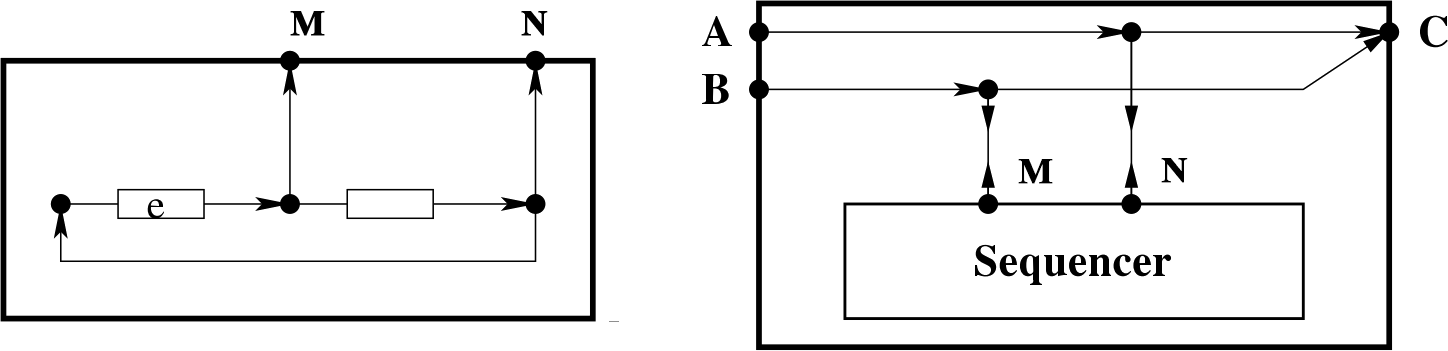
\includegraphics[width=.9\textwidth]{images/reoexample.png}
    \caption{How A Sequencer Connector is Defined and Reused in Reo \cite{MengReoUml2011}}
    \label{fig:reoexample}
\end{figure}

Inspired by Reo, we present a new modeling language, \lang{}. \lang{} is a hierarchical modeling language that provides formalism for both high-level \emph{system} layouts and low-level \emph{automata}-based behavioral units. With help of a rich-featured type system, we can describe complex data structure and powerful automata in a rather formal way. And automata (or other systems) can be then declared as either components or connectors in a system. Both automata and systems are encapsulated with a interface containing \emph{a) a set of input or output ports} and \emph{b) a set of template parameters} so that they can be easily reused in multiple projects. 

The paper is structured as follows. In Section \ref{sec:syntax}, we briefly present the syntax of \lang{} and formalizations of the language entities. Then in Section \ref{sec:semantics}. we introduce the formal semantics of \lang{}. Section \ref{sec:casestudy} presents a case study where a commonly used coordination algorithm \emph{leader election} is modeled in \lang{}. The conclusion and future work can be found in Section \ref{sec:conclusion}.